\label{subsec:experimental_analysis}
In the previous section, we outlined our basic algorithm and illustrated its results that
show superior performance compared to state-of-the-art on three datasets. In this section
we analyze various components of our algorithm to illustrate how 
our approach performs under different settings. Detailed results are provided in the website.

\textbf{Runtime} For both approaches, candidate algorithms can be run in parallel and hence
the total time taken by them on an input image is the maximum time of any algorithm. As an overhead,
we compute SIFT/HOG based features on the output of these algorithms, which measures in milliseconds
since fast GPU based approaches are available for such computations. On top of that, the output selection 
part uses Euclidean distance computation for kNN, which amounts to 5 (candidate algorithms) x 20
(exemplars) distance computations between 535 dimensional vectors (of SIFT/HOG features). 
Finally, the optimization algorithm takes 0.4 seconds to converge for a single input image on a 
Intel(R) Xeon(R) CPU E5-2640 0 @ 2.50GHz system.

\textbf{SIFT vs HoG}
\label{subsec:sift_vs_hog_vs_both}
%Algorithm~\ref{alg:feature_computation} outlines our approach to compute SIFT and HOG features
%around fiducial locations in a face image. In this experiment, we contrast the contribution of SIFT
In this experiment, we contrast the contribution of SIFT
and HOG features for the task of output selection. Results of our experiment comparing mean errors
and failure rates on all datasets are shown in Figure~\ref{fig:sift_vs_hog}. Note that
SIFT outperforms HOG, and understandably so since SIFT captures appearance details lost to HOG. 
We get an improvement of $6\%$ using SIFT and $2\%$ using HOG over competing
methods.
% Algorithm~\ref{alg:feature_computation} outlines our approach to compute SIFT and HOG features
% around fiducial locations in a face image. In this experiment, we try to determine the contribution
% of each type of feature to the basic output selection algorithm. In order to do this, we
% perform two experiments. In the first experiment, we compute feature vectors around each fiducial
% consisting of only SIFT features at the two scales previously mentioned. In the second experiment,
% we compute HOG features instead of SIFT. Note that exemplar selection in the basic algorithm is
% not affected by this change of features since it is only shape dependent. Results of our experiment
% comparing mean errors on the COFW dataset are shown in Figure~\ref{fig:sift_vs_hog}. Note that
% while SIFT performs better than HOG, our basic algorithm that uses both SIFT and HOG features 
% generally does better than both. We get an improvement of $6\%$ using SIFT over other competing
% methods and an improvement of $2\%$ using HOG.

\begin{figure}
  \centering
  \subfloat[ ]{
  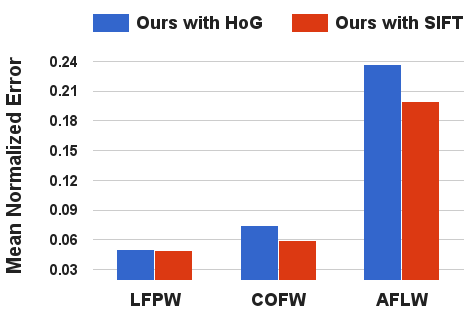
\includegraphics[width=3.2in,height=2.5in]{fid/figures/hogvsift/mean_normalized_error.png}}
  \subfloat[ ]{
  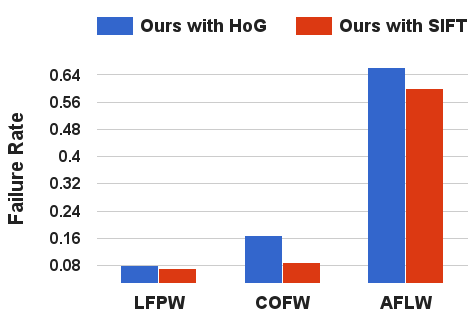
\includegraphics[width=3.2in,height=2.5in]{fid/figures/hogvsift/failure_rate.png}
  \label{fig:sift_vs_hog}}
  \\
  %\subfloat[ ]{
  %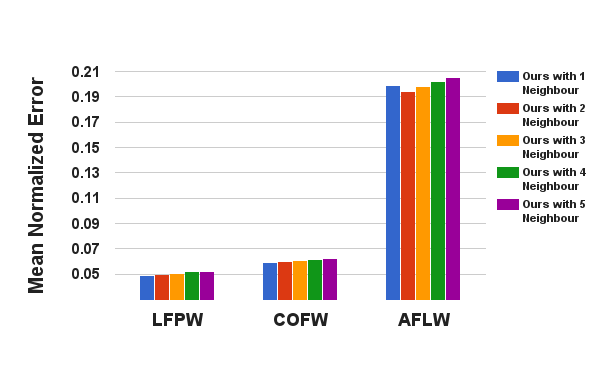
\includegraphics[width=1.35in,height=1.1in]{figures/knn/mean_normalized_error.png}}
  %\subfloat[ ]{
  %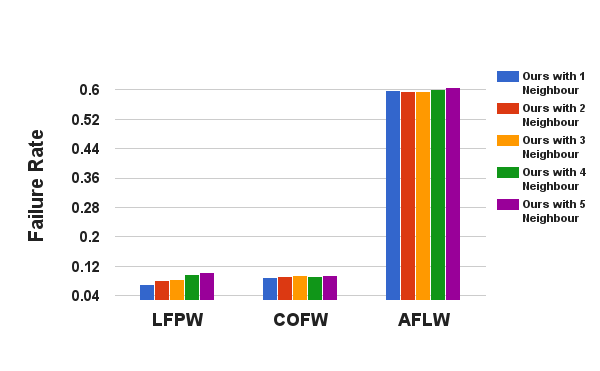
\includegraphics[width=1.35in,height=1.1in]{figures/knn/failure_rate.png}
  %\label{fig:nearest_neighbors}}
  %\caption{ Comparison of mean error and failure rate for (a,b) SIFT vs HOG experiment and (c,d)
  %nearest neighbor experiment for $k = \{1, 2, 3, 4, 5\}$. Note that $k=1$ represents the basic algorithm. 
  %Best viewed in color.}
  \caption{ Comparison of mean error and failure rate for SIFT vs HOG experiment.
  Best viewed in color.}
\end{figure}

% \paragraph{Optimization vs kNN}
% Table~\ref{table:by_parts} shows the comparitive result between method
% described in earlier section and this method for LFPW dataset. 
%  \begin{table}[!h]
%     \centering
%     \begin{tabular}{lcc}
%     \toprule[1.5pt]
% %     \specialcell{\bf Dataset} &  \specialcell{\bf Chehra} &  \specialcell{\bf \textcolor{red}{Zhu}} &  \specialcell{\bf Intraface} &  \specialcell{\bf RCPR} &  \specialcell{\bf Ours} \\
%      \bf Metric &  \bf Method as whole&  \bf By parts  \\
%     \midrule
%     \bf Failure Rate & 7.21 & 9  \\
%     \bf Mean Error & 4.89 & 5.7  \\
%     \bottomrule[1.5pt]
%     \end{tabular}
%     \caption{Comparision between "Method as whole" and "By parts".}
%     \label{table:by_parts}
% \end{table}
 
 
% \begin{figure}
%   \centering
%   \caption{ Best viewed in color.}
% \end{figure}
%  

% \paragraph{Varying Selection Neighborhood}
% \label{subsec:nearest_neighbors}
% Each candidate in $\mathcal{O}_{all}$ in Algorithm~\ref{alg:output_selection} is ``tagged'' with 
% its distance (stored in the variable $dist_i$) from the \emph{nearest} exemplar. 
% We could alternatively tag each candidate with the sum of distances from $k$ nearest neighbors.
% This approach represents a trade-off between accuracy and robustness, since the \emph{nearest} exemplar
% is almost always of similar pose and thus lends to better pixel accuracy of fiducial features, 
% while using $k > 1$ \emph{nearest} exemplars results in better robustness to partial occlusion.
% Figure~\ref{fig:nearest_neighbors} shows the result of our algorithm on COFW, when the number
% of neighbors is varied from $1$ to $5$. Note that increasing neighbors degrades both mean error
% and failure rates, indicating robustness to partial occlusion is the lesser of the two problems.
% 
% % Once feature computations and distances between fiducials have been computed 
% % for a test image in Algorithm~\ref{alg:output_selection}, each result in $\mathcal{O}_{all}$ is ``tagged'' with its
% % distance from the \emph{nearest} exemplar (The variable $dist_i$ stores this
% % information). This approach represents a trade-off between accuracy
% % and robustness. On the one hand, given that exemplars vary significantly in various 
% % aspects like pose, expression, texture, etc. choosing more than one nearest exemplar might
% % dilute the similarities of shape and appearance of these exemplars and the test image.
% % Thus choosing lesser number of exemplars leads to higher accuracy. On the other hand, partial
% % occlusion is better bypassed when several exemplars are involved in distance computation.
% % 
% % Figure~\ref{fig:nearest_neighbors} shows the result of our algorithm on COFW, when the number of neighbors used in selecting
% % the best output vary from 1 to 5. Note that both the mean and the failure rate increase slightly
% % with the number of neighbors, consistent with the fact that there is an accuracy decrease when
% % more than 1 exemplars are used to select one output. We also argue that in
% % test images of this dataset, partial occlusion does not result in majority of the fiducials being
% % occluded, and thus the first nearest neighbor selected is still very accurate with respect to pose and appearance
% % variation.                                                                     
% 
\textbf{Varying Number of Exemplars}
\label{subsec:varying_number_of_exemplars}
Varying the number of exemplars ideally affects the accuracy of fiducial location, since
more exemplars should typically mean that the nearest neighbor
 should be more similar to the test image. However if most
variations in pose, expression, partial occlusion have been already captured, increasing the number
of exemplars will have minimal effect on accuracy. This is precisely what we observe in
Figure~\ref{fig:num_exemplars}.

\textbf{Optimization with structural costs}
\label{subsec:with_without_structural_costs}
In this experiment, we show qualitative result of output selection by optimization with and without
structural costs. Structural costs help in optimizing to a solution which looks like face. If only
appearance costs are used, it leads to just selecting best looking fiducials individually leading to distortion in facial structure which can be observed in third image of Figure~\ref{fig:with_without_structural_costs}.

\begin{figure}
  \centering
  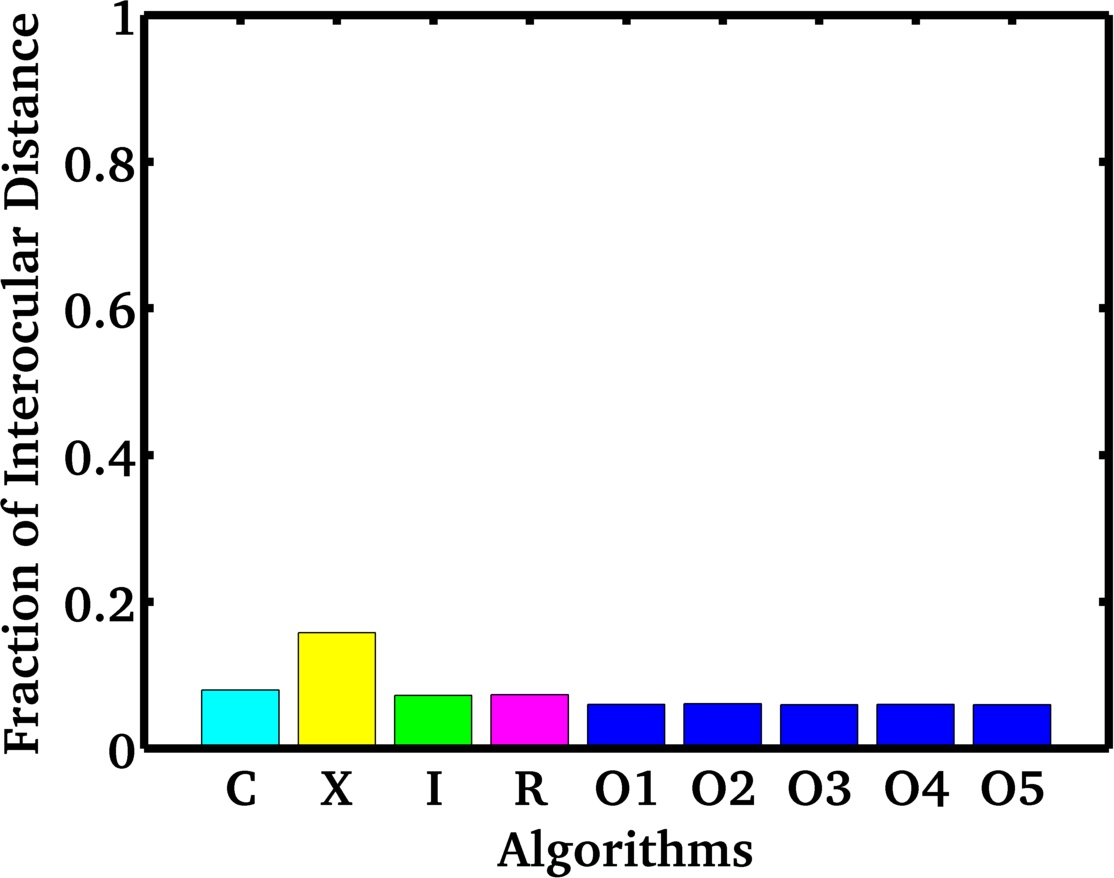
\includegraphics[width=3.0in,height=2.5in]{fid/figures/iccv_version_one/cofw/num_of_exemplars/mean_err_modified.jpg}
  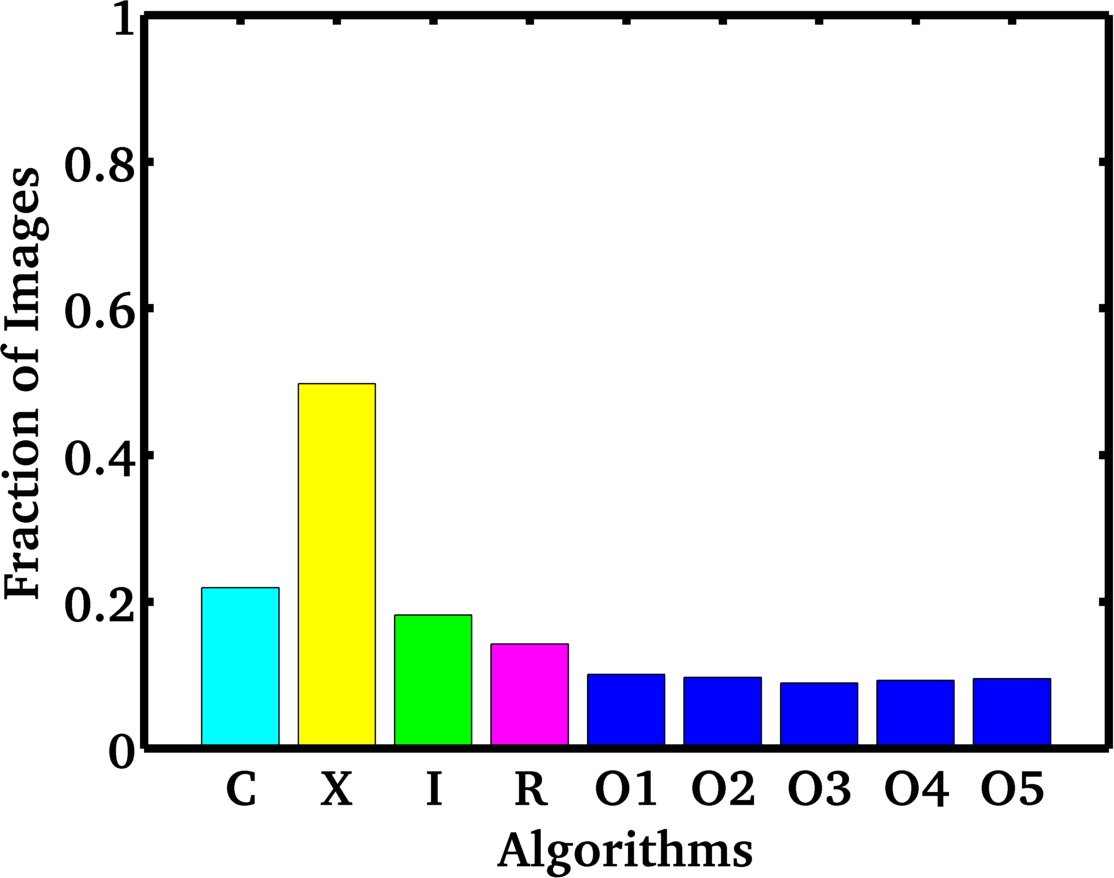
\includegraphics[width=3.0in,height=2.5in]{fid/figures/iccv_version_one/cofw/num_of_exemplars/fail_rate_modified.jpg}
  \caption{ Comparison of mean error and failure rate when the number of exemplars is increased.
  Results O1-O5 correspond to our algorithm with number of exemplars (20, 30, 40, 50, 60) respectively. 
  C, X, I and R corresponds to Chehra, Deva, Intraface and RCPR respectievely.
  Best viewed in color. }
  \label{fig:num_exemplars}
\end{figure}

% % \subsection{Manual vs Automatic Selection}
% % \label{subsec:manual_vs_automatic}
% % Manual vs automatic experiment.
 
\textbf{Shape vs Appearance}
\label{subsec:shape_vs_appearance}
Algorithm~\ref{alg:exemplar_selection} outlines our approach of using both shape specific and
appearance specific exemplars in output selection. In this experiment, we measure the relative
importance of each type of exemplar. Figure shows results of our
experiment, where we find that both have almost equal contributions to the superiority of 
output selection in comparison to competing methods.
% % In Algorithm~\ref{alg:exemplar_selection}, we outline our approach to compute shape specific and
% % appearance specific exemplars that clusters images and fiducials in the training set using kmeans
% % and selects one exemplar per cluster. While the basic approach outlined in
% % section~\ref{subsec:basic_algorithm} uses \emph{both} sets of exemplars for output selection, we
% % measure the relative importance of each type of cue in this experiment.
 
Figure~\ref{fig:kmeans_vs_pca} shows our results when only one type of exemplars are used
for output selection on the COFW dataset. Shape based and appearance based exemplars perform in a complimentary manner.
Shape based exemplars provide robustness to partial occlusion, since they are better at identifying
non-occluded fiducials, and generally result in nearest neighbors that are closer in pose to the
test image. On the other hand, while appearance based exemplars falter in the presence of occlusion,
they are better at identifying more accurate fiducials when all candidate algorithms give accurate outputs.

 \begin{figure}
  \centering
  \subfloat[]{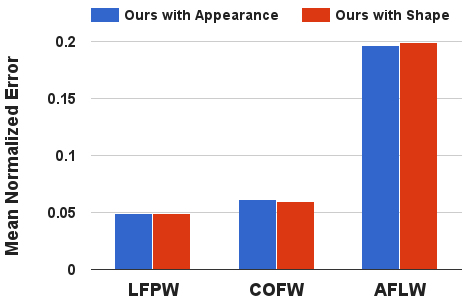
\includegraphics[width=3.2in,height=2.5in]{fid/figures/shapevsapp/mean_error.png}\label{fig:sva_shape_mean}}
  \subfloat[]{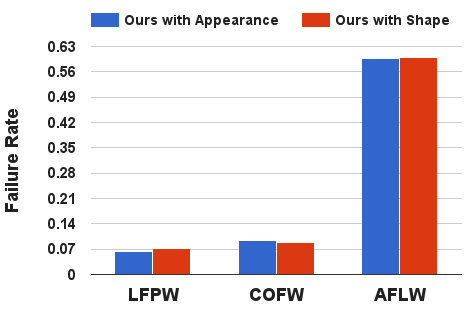
\includegraphics[width=3.2in,height=2.5in]{fid/figures/shapevsapp/failure_rate.png}\label{fig:sva_shape_fail}}
  \caption{ Comparison of mean error and failure rates for the shape vs appearance experiment. Best viewed in color. }
  \label{fig:shape_vs_appearance}
\end{figure}

% %\paragraph{Illumination Normalization}
% %\vspace{1in}
 
\textbf{Clustering vs Eigenspace Analysis}
\label{subsec:clustering_vs_eigenspace}
While {\tt kmeans} has been the preferred choice of clustering method for
Algorithm~\ref{alg:exemplar_selection}, we also experimented with using principal component
analysis (PCA) instead. In order to select exemplars using PCA, we construct a shape matrix
where each column represents an exemplar, and find its top $20$ principal components. We then
select one exemplar per component such that it maximizes its dot product with the corresponding
principal component. Results, show negligible difference
between the two approaches. We repeated the same experiment with appearance exemplars with similar
results.
% % In the previous experiment, we compared the effect of shape based and appearance based exemplars on
% % output selection. Both these exemplars are currently selected using kmeans as illustrated in
% % Algorithm~\ref{alg:exemplar_selection}. However, an alternate approach to capture variation in
% % exemplars is to project them into a lower dimensional subspace, and select samples that are
% % orthogonal to each other (and hence complimentary). More specifically, we concatenate shape (x, y
% % locations) and appearance (sift/hog features) for each exemplar into a matrix and perform a
% % principal component analysis (PCA) to select the top $k$ (20 in this case) eigenvectors. We then choose
% % one exemplar per eigenvector such that the dot product of the exemplar and the eigenvector is
% % maximized. We can then alternatively use these exemplars in place of exemplars produced by kmeans
% % for output selection (Algorithm~\ref{alg:output_selection}).
% % 
% % Figure~\ref{fig:shape_vs_appearance} illustrates results when we use kmeans (labeled $O1$)
% % vs when we use PCA (labeled $O2$) on the COFW dataset.
% % Figures~\ref{fig:sva_shape_mean},\ref{fig:sva_shape_fail} show results when using shape based
% % exemplars, and figures~\ref{fig:sva_app_mean}, \ref{fig:sva_app_fail} show results when using 
% % appearance based exemplars. Overall, we found that kmeans performs slightly better with respect to
% % failure rates, while mean errors are similar in both cases. Additional results can be found in the
% % supplementary material.
% 
\begin{figure}
  \centering
  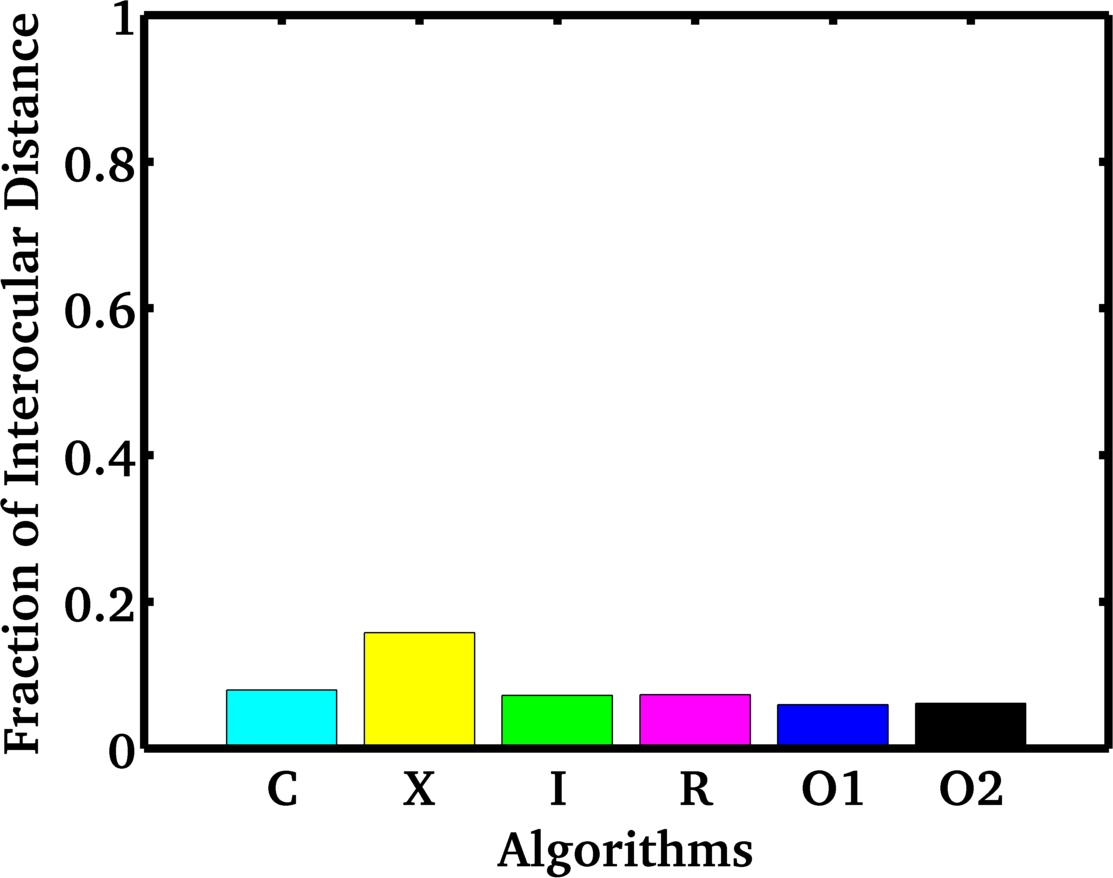
\includegraphics[width=3.0in,height=2.5in]{fid/figures/iccv_version_one/cofw/kmeans_shape_vs_kmeans_pca/mean_err_modified.jpg}
  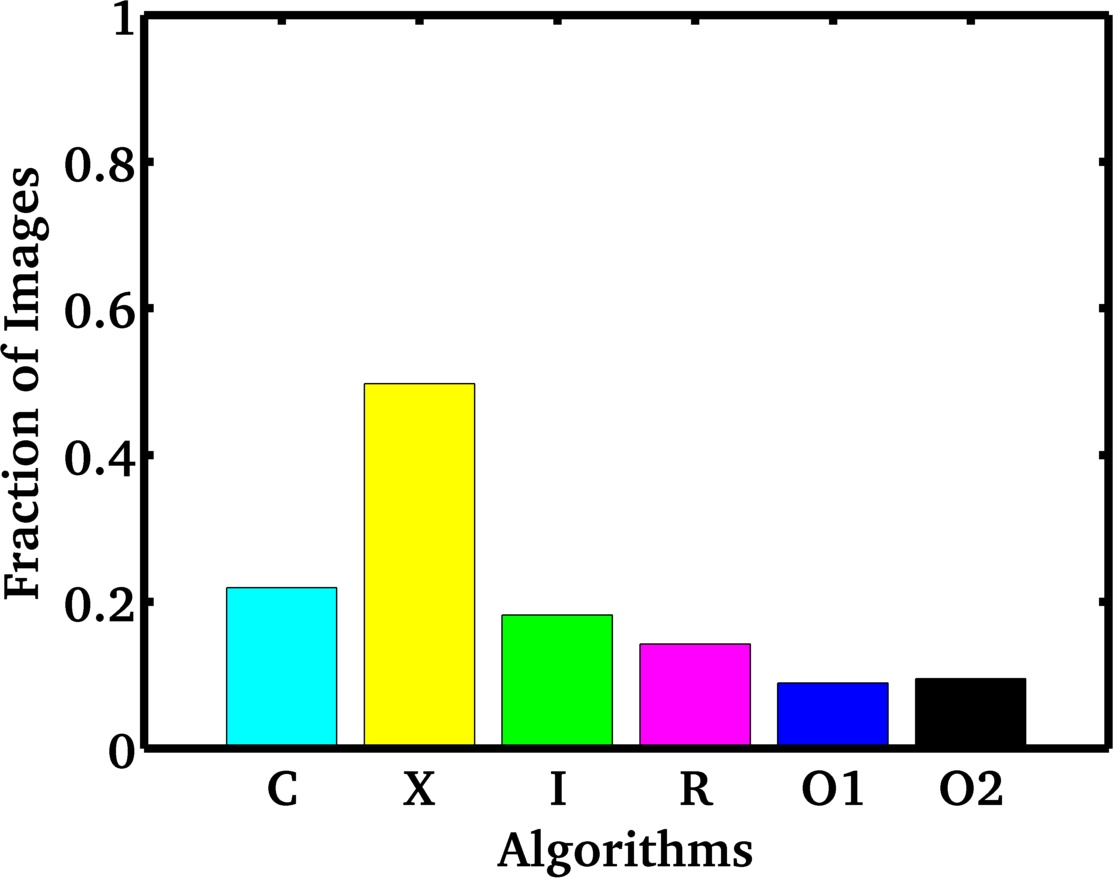
\includegraphics[width=3.0in,height=2.5in]{fid/figures/iccv_version_one/cofw/kmeans_shape_vs_kmeans_pca/fail_rate_modified.jpg}
  \caption{ Comparison of exemplars for kmeans vs PCA. O1 represents our basic result and O2
  represents PCA based results. Best viewed in color 
  C, X, I and R corresponds to Chehra, Deva, Intraface and RCPR respectievely. }
  \label{fig:kmeans_vs_pca}
\end{figure}
% 
% %%%  \begin{table}
% %%%   \begin{tabular}{|c|c|c|c|c|c|}
% %%%     \hline 
% %%%     &  Deva & Intraface & Chehra & RCPR & Ours \\
% %%%     \hline 
% %%%   \end{tabular}
% %%%   \caption{Results on the COFW dataset.}
% %%% \end{table}  
% 

\textbf{Euclidean distance vs Metric Learning}
\label{subsec:euc_vs_metric}
We also performed an experiment to compare the performance of our algorithm when we use euclidean distance and
Mahalanobis distance to find the similarity score between candidate results on a test image and exemplars. 
We learn the transformation matrix based on~\cite{weinberger09distance}. Metric is learnt with the objective of
minimizing the distance of $k$ nearest samples belonging to same class in the transformed domain and
maximizing if the samples are of different class. Here we compute transformation matrix for each of
the part in one vs rest fashion. Appearance feature vector (SIFT and HoG) computed given the ground
truth location for a part is considered to be of one class and appearance feature vector of other
parts are considered to be of another class. Transformation matrix is learnt. Learnt matrix is used
to compute the similarity score for each of the part prediction in the test sample with the part in
the exemplar. We use 200 samples for each part with the feature dimension of 535. 
We note that insignificant improvement is obtained using metric learning.
Figure ~\ref{fig:metric_learning} shows the failure rate analysis of different datasets. 
We believe since the appearance representation of fiducials are too diverse for the metric to capture
meaningful statistical information, metric learning failed to perform better than the simple Euclidean metric.

%We see similarity score computed
%using Euclidean distance performs consistently better compared to Mahalanobis distance. Also observe
%that the more challenging the dataset gets, worse the failure rate using Mahalanobis distance. Hence
%exemplar methods are more suitable with Euclidean distance as compared to Mahalanobis distance as it
%tries to generalize across variation. 

\begin{figure}
  \centering
  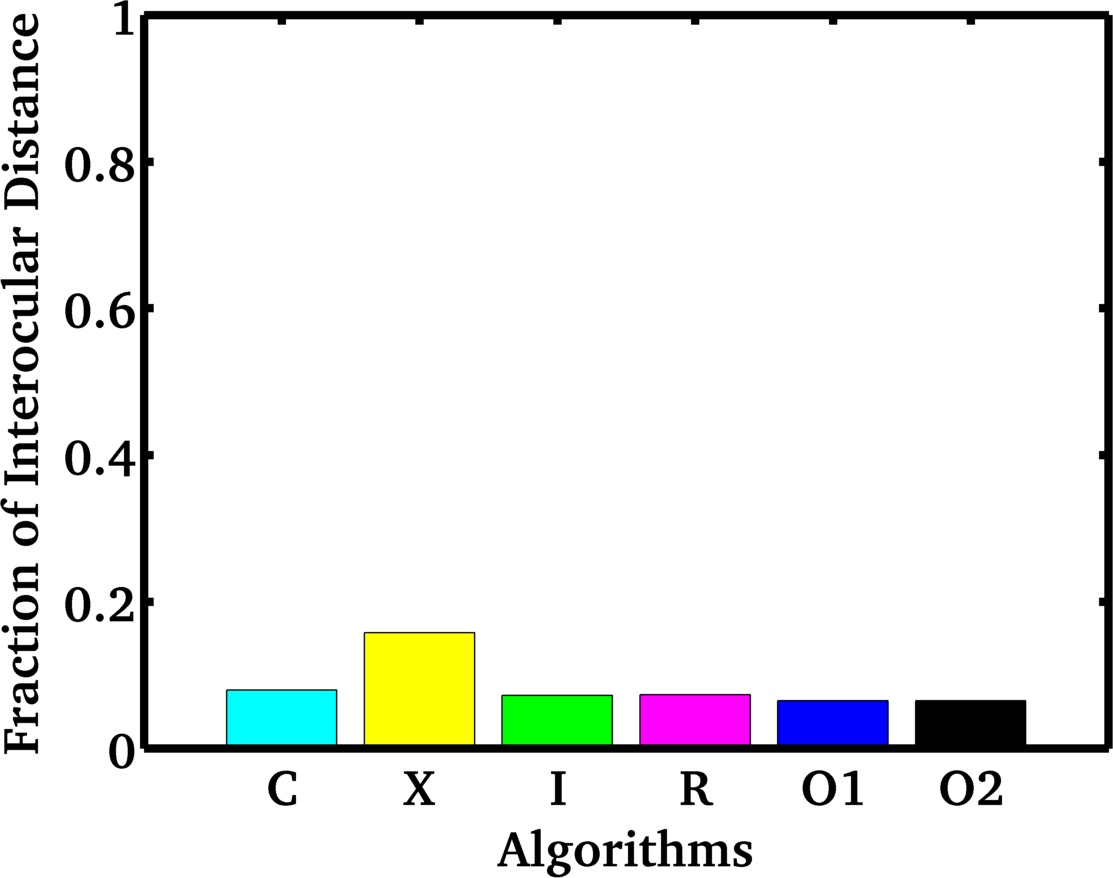
\includegraphics[width=3.0in,height=2.5in]{fid/figures/iccv_version_one/cofw/wo_metric_vs_w_metric/mean_err_modified.jpg}
  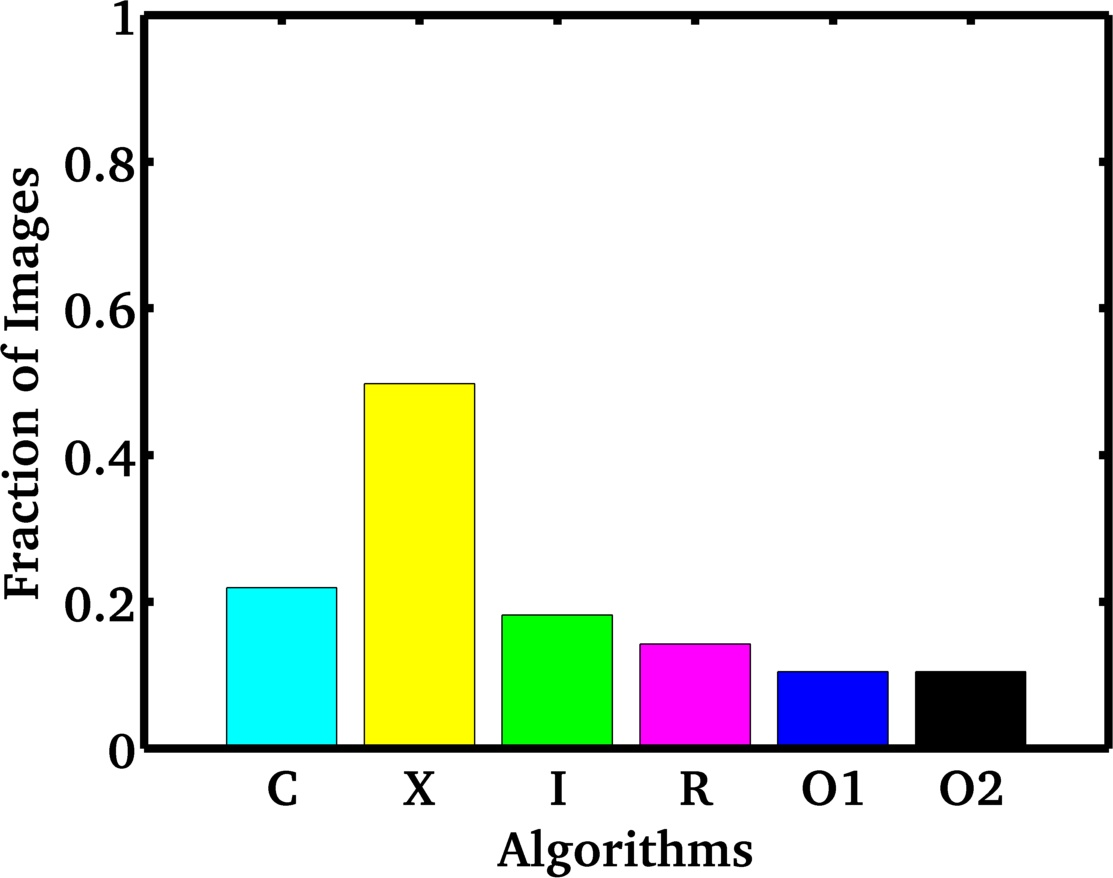
\includegraphics[width=3.0in,height=2.5in]{fid/figures/iccv_version_one/cofw/wo_metric_vs_w_metric/fail_rate_modified.jpg}
  \caption{ Comparison of Metric Learning Result. O1 represents our results with Euclidean metric and O2 with learnt metric.
  C, X, I and R corresponds to Chehra, Deva, Intraface and RCPR respectievely.
  }
  \label{fig:metric_learning}
\end{figure}
